\section{Anwendungsfälle}

\subsection{Rezeptverwaltung}
\begin{figure}[H]
	\begin{center}

	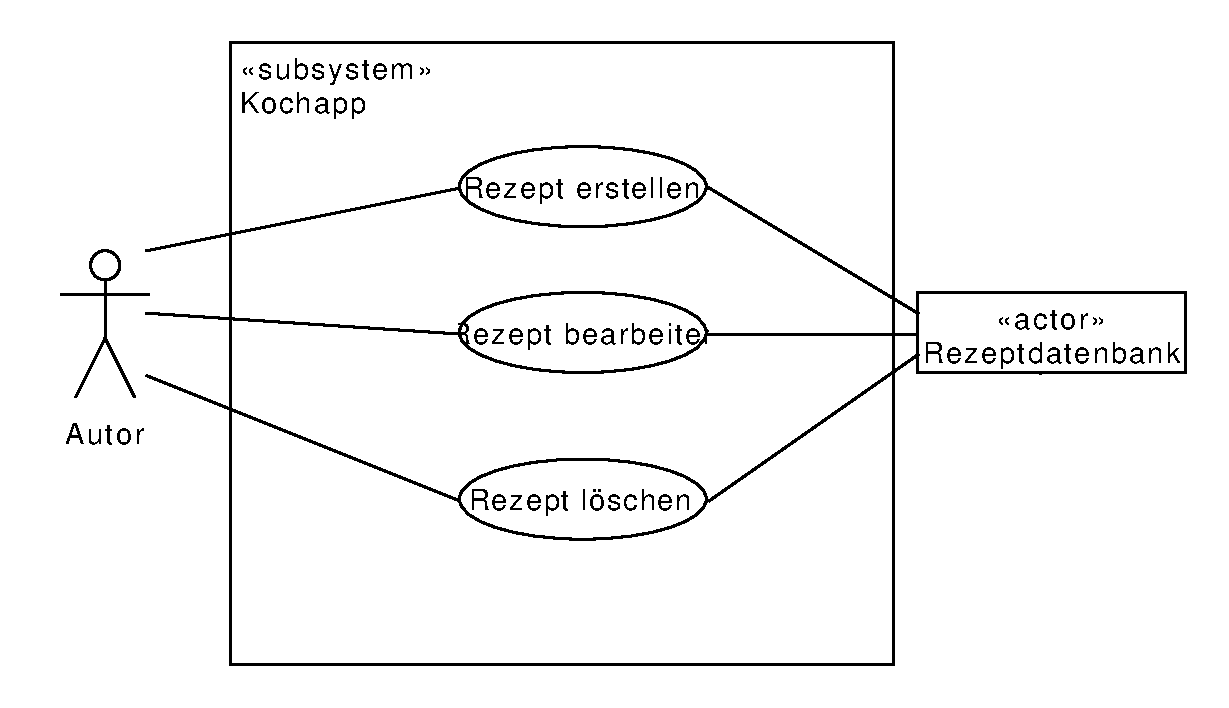
\includegraphics[width=0.8\textwidth]{grafiken/Anwendungsfalldiagramm_Rezeptverwaltung.pdf}
	\caption{Rezeptverwaltung von einem Autor}
		\end{center}
\end{figure}

\subsection{Interaktion mit öffentlichen Rezepten}
Im folgenden Diagramm wird die Interaktion mit öffentlichen Rezepten verdeutlicht. Ein Nutzer in der Rolle als \gls{Autor} publiziert sein privates Rezept, damit ist es als öffentliches Rezept verfügbar. Als \gls{Autor} kann er es auch wieder entfernen. 
Ein Nutzer in der Rolle als Rezeptsuchender kann es favorisieren, damit ist es bei ihm gespeichert. Er kann bewerten oder kommentieren. 

\begin{figure}[H]
\begin{center}
	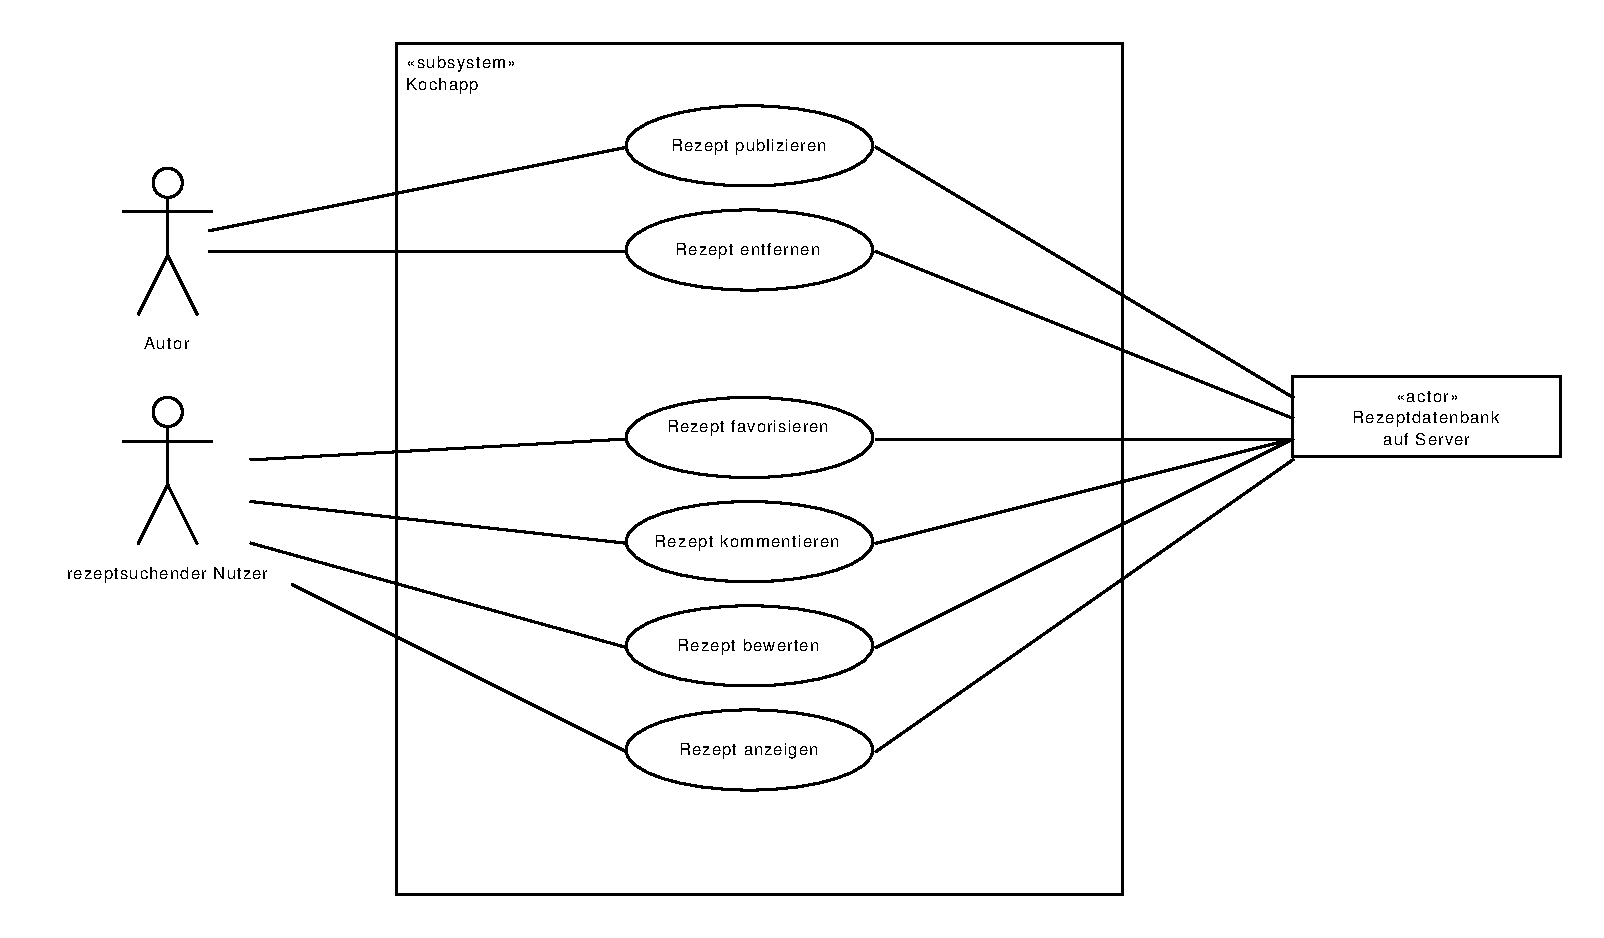
\includegraphics[width=1.0\textwidth]{grafiken/Anwendungsfalldiagramm_oeffentliche_Rezeptverwaltung.pdf}
	\caption{Aufgaben die ein Autor und ein rezeptsuchender Nutzer durchführen kann}
\end{center}
\end{figure}


\subsection{Benutzerverwaltung}
\begin{figure}[H]
\begin{center}
	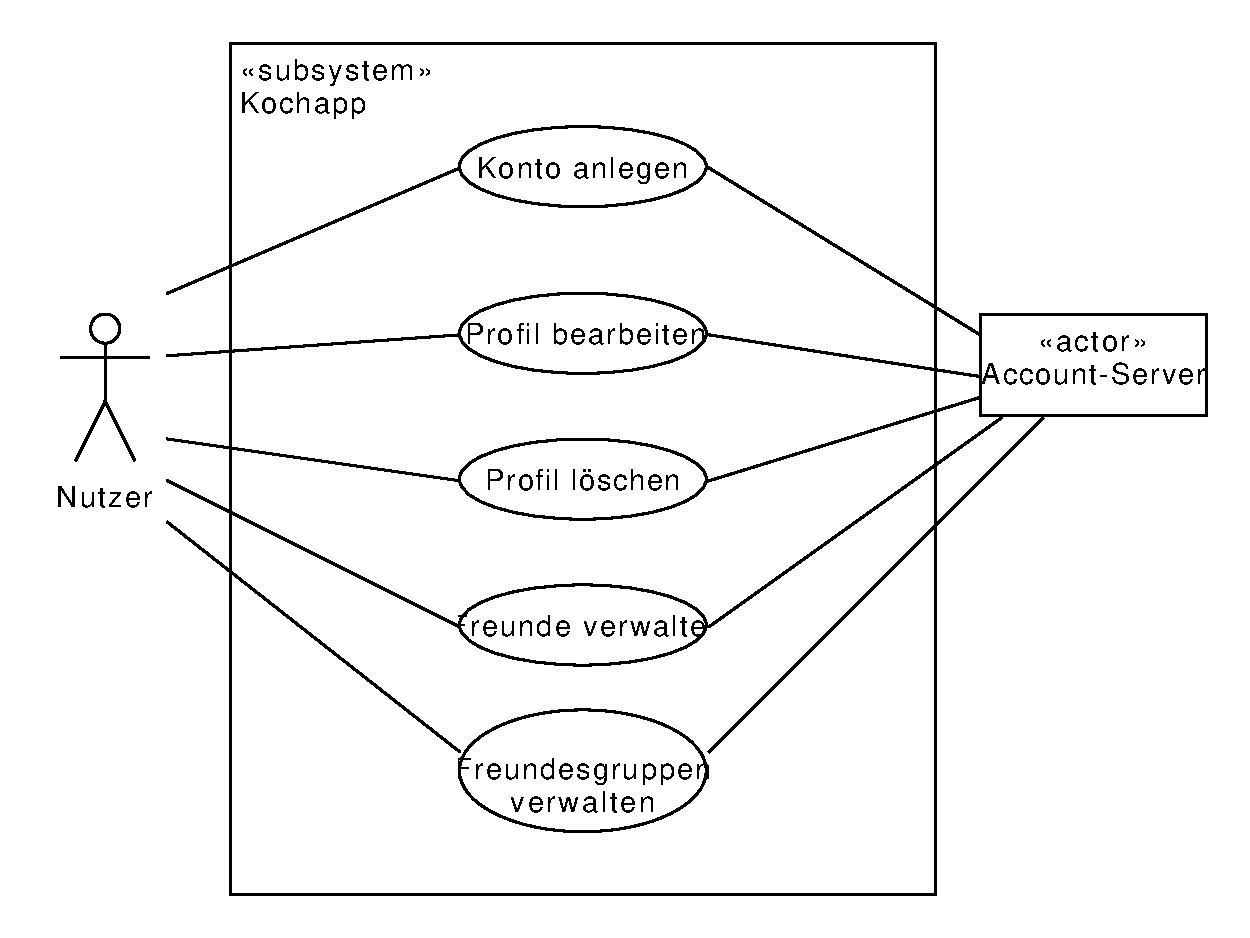
\includegraphics[width=0.8\textwidth]{grafiken/Anwendungsfalldiagramm_Benutzerverwaltung.pdf}
	\caption{Benutzerverwaltung eines Nutzers}
\end{center}
\end{figure}


%\subsection{Rezeptsuche}
%Todo suche noch in neues Diagramm oben eintragen. 
%\begin{center}
%	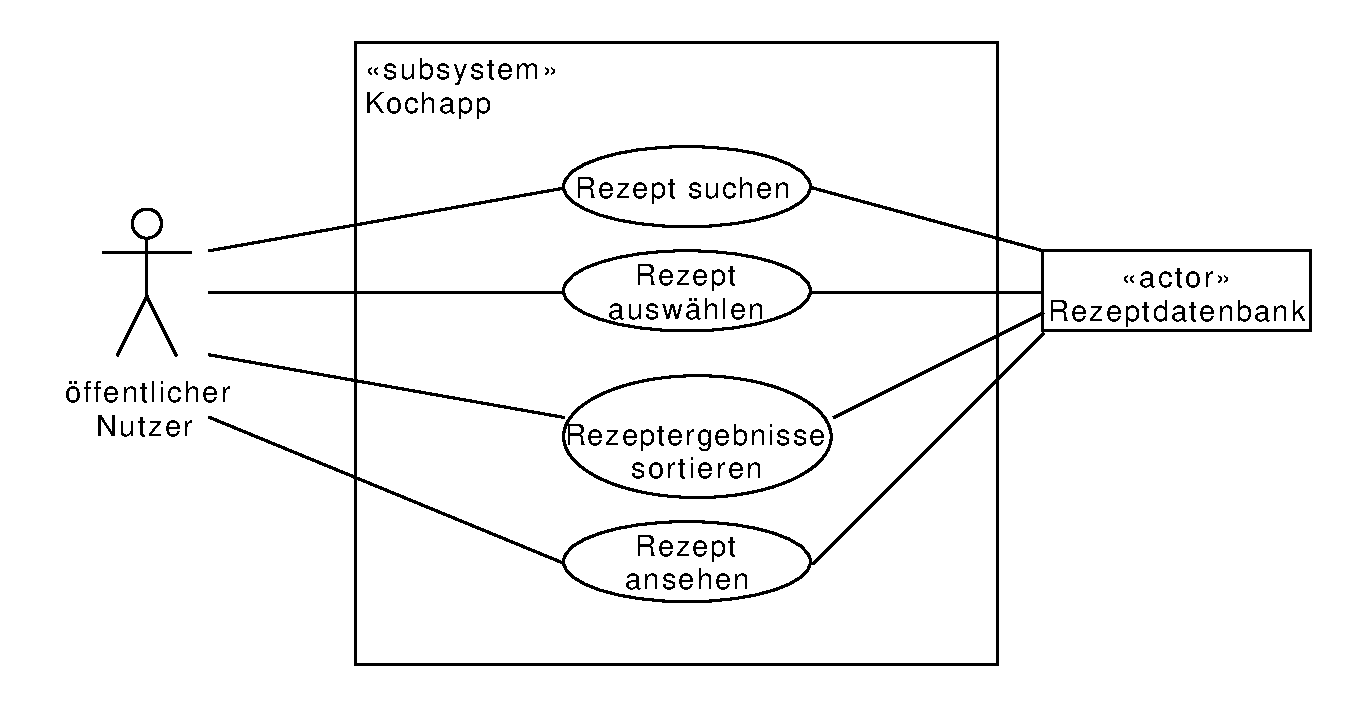
\includegraphics[width=0.8\textwidth]{grafiken/Anwendungsfalldiagramm_Rezeptsuchen.jpg}
%\end{center}



